\documentclass{beamer}

\def\Tiny{\fontsize{6pt}{6pt}\selectfont}
\def\supertiny{\fontsize{4pt}{4pt}\selectfont}

\mode<presentation>
{
  \usetheme{Warsaw}
  % \setbeamercovered{transparent}
  \usecolortheme{crane}
}

\usepackage{graphicx, ifthen, listings, fancyvrb}

\usepackage[czech]{babel}
% \usefonttheme{professionalfonts}
\usepackage{times}
\usepackage{amsmath}
\usepackage[utf8]{inputenc}
\usepackage{wrapfig}

\usepackage[T1]{fontenc}

\lstset{ basicstyle=\tiny, stringstyle=\ttfamily, showstringspaces=false }

\everymath{\displaystyle}

\setbeamerfont{frametitle}{size=\large}
\setbeamerfont{subsection in toc}{size=\scriptsize}

\makeatletter\newenvironment{blackbox}{%
   \begin{lrbox}{\@tempboxa}\begin{minipage}{0.95\columnwidth}}{\end{minipage}\end{lrbox}%
   \colorbox{black}{\usebox{\@tempboxa}}
}\makeatother

\title[IMF (9)]{Informatika pro moderní fyziky (9)\\ procvičení datových vazeb, CSS - stylování dokumentů, SVG - tvorba obrázků, složitější interaktivní dokument}

\author[Franti\v{s}ek HAVL\r{U}J, ORF ÚJV Řež]{Franti\v{s}ek HAVL\r{U}J\\{\scriptsize \emph{e-mail: haf@ujv.cz}}}

\date{akademický rok 2015/2016\\8. prosince 2015}

\institute[ORF ÚJV Řež]
{ÚJV Řež\\oddělení Reaktorové fyziky a podpory palivového cyklu}

\AtBeginSection[]
{
\begin{frame}<beamer>
\frametitle{Obsah}
\tableofcontents[currentsection,hideothersubsections]
\end{frame}
}

\begin{document}

\begin{frame}
  \titlepage
\end{frame}

\begin{frame}
  \tableofcontents
\end{frame}

\section{Co jsme se naučili minule}

\begin{frame}{}
  \begin{itemize}
    \item opět zpracování dat
    \item JS pro běžné použití (toggle)
    \item procvičení ERb -- skládání většího HTML dokumentu
  \end{itemize}
\end{frame}

\section{Stylování dokumentů}

\begin{frame}{CSS}
  \begin{itemize}
    \item jazyk pro popis vzhledu HTML dokumentu
    \item v nejjednodušším přístupu definuje styly pro jednotlivé typy elementů
    \item dále umožňuje definovat tzv. třídy (skupiny elementů, pomocí atributu \texttt{class} v HTML) a také styly pro konkrétní elementy (id)
    \item složitější selekory -- vnoření, souslednost atd.
  \end{itemize}
\end{frame}

\begin{frame}[fragile]{CSS - jednoduchý příklad}
  \begin{itemize}
    \item základní selektory: \emph{element}, \emph{.třída} a \emph{\#id}
    \item základní syntaxe \emph{vlastnost: hodnota;}
  \end{itemize}
  \scriptsize
  \begin{verbatim}
    a {
      color: blue;
      text-decoration: none;
      font-weight: bold;
    }
    #core_map { float:left; }
  \end{verbatim}
\end{frame}

\begin{frame}{CSS - kam s ním}
  \begin{itemize}
    \item přímo k tagu (\texttt{<div style=``display:none''>}) -- možná dobré na rychlé ladění/patlání, ale vesměs vždy špatně; jedinou výjimkou je \texttt{display:none} pro elementy, které mají být vidět až později, tam to jinak nejde
    \item v hlavičce (\texttt{head}) HTML dokumentu: \texttt{<style type=``text/css''>...</style>}
    \item v externím souboru (obvykle jediné správné řešení) -- pomocí tagu \texttt{link} v hlavičce
    \item my vystačíme se \texttt{style} tagem v hlavičcce
  \end{itemize}
\end{frame}

\begin{frame}{Rychlé procvičení}
  \begin{itemize}
    \item vezměte si svoje krásné HTML z minula a doplňte do něj trochu toho stylování
    \item minimum: změnit font (\texttt{font-family}), nastavit rozumné velikosti písma a barvy
    \item zrušit podtrhávání odkazů (\texttt{text-decoration})
    \item bonus: jiná barva odkazů na přepínání tabulka/graf
  \end{itemize}
\end{frame}

\section{Tvorba obrázků}

\begin{frame}{Zadání dnešní úlohy}
  \begin{itemize}
    \item každý den data z 1-9 detektorů (\texttt{data/*.csv})
    \item detektor má svoji polohu v AZ (VR-1 Vrabec, 8x8 čtvercových pozic) -- včetně data je uvedena na prvním řádku CSV souboru
    \item je potřeba hezky zobrazit na každý den mapu AZ a grafy signálů z detektorů
    \item viz \texttt{html/document.html}
  \end{itemize}
\end{frame}

\begin{frame}{Jak na obrázky}
  \begin{itemize}
    \item pěkný formát na tvorbu vektorových obrázku je SVG (Scalable Vector Graphics)
    \item je to dobrá věc především na internet -- všechny prohlížeče ho umí
    \item stejně jako HTML je postaven na XML, takže už to vlastně umíme
  \end{itemize}
\end{frame}

\begin{frame}[fragile]{Jednoduchý příklad}
  \tiny
  \begin{verbatim}
    <svg width="320" height="320" xmlns="http://www.w3.org/2000/svg" version="1.1">
      <rect x="0.0" y="0.0" width="40.0" height="40.0" fill="blue" />
      <rect x="40.0" y="0.0" width="40.0" height="40.0" fill="red" />
      <rect x="0.0" y="40.0" width="40.0" height="40.0" fill="green" />
      <rect x="40.0" y="40.0" width="40.0" height="40.0" fill="yellow" />
    </svg>
  \end{verbatim}
  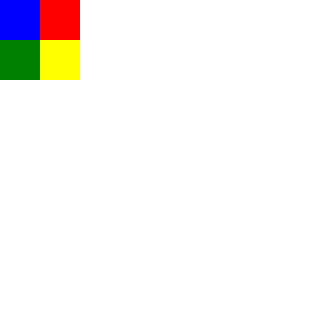
\includegraphics[width=0.15\textwidth]{example}
\end{frame}

\begin{frame}{SVG -- co a jak}
  \begin{itemize}
    \item souřadný systém z levého horního rohu
    \item je potřeba udat celkovou šířku a výšku
    \item zatím nám stačí obdélník -- tag \texttt{rect}
    \item pozor, je to striktní XML, tedy je nutné \texttt{rect} tag uzavřít (!)
    \item vyzkoušejte -- nejdřív jen tak, potom vygenerovat 8x8 mapu (zatím klidně prázdnou)
  \end{itemize}
\end{frame}

\begin{frame}{Jak vložit do HTML}
  \begin{itemize}
    \item jsou různé metody, jak vložit ze souboru
    \item my se bez toho v pohodě obejdeme - vložíme přímo (\texttt{IO.read})
    \item v tu chvíli je totiž mj. možné naplácat na SVG objekty javascriptové handlery
    \item ... tedy na čtverečku můžu mít onclick
  \end{itemize}
\end{frame}

\begin{frame}{Zpracovat data}
  \begin{itemize}
    \item pro každý CSV soubor chceme mít graf (gnuplot/png)
    \item pro každý den mapu (nejdřív obyčejnou, potom klikací, pak třeba s textem)
  \end{itemize}
\end{frame}

\begin{frame}{Další JS chytrosti}
  \begin{itemize}
    \item v jQuery už známe \texttt{\$(`\#id')}
    \item ale ve skutečnosti jde použít jakýkoli CSS selektor, takže třeba \texttt{\$(`p')}
    \item pokročilý CSS selektor -- vnoření: \texttt{\#my\_list img} vybere všechny obrázky (\texttt{img}) které jsou uvnitř elementu s id \texttt{my\_list}
    \item ... použiju v situacích, kdy chci schovat nějakou množinu elementů a pak jeden z nich zobrazit (tj. když mám hromadu obrázků a chci, aby byl vidět jen jeden)
  \end{itemize}
\end{frame}

\begin{frame}{Další CSS chytrosti}
  \begin{itemize}
    \item normálně se jednotlivé elementy řadí pod sebe
    \item můžu místo toho použít tzv. floating, kdy se začnou elementy řadit nalevo nebo napravo
    \item efekt znáte např. z webových galerií, kde mi fotky vyplní celou šířku okna a jdou po řádcích
    \item \texttt{float:left}
    \item barvu pozadí nastavím např. \texttt{background-color:red} nebo \texttt{background-color:\#ddddff}
  \end{itemize}
\end{frame}


\begin{frame}{Další SVG chytrosti}
  \begin{itemize}
    \item kromě \texttt{rect} se bude hodit také \texttt{text}
    \item jako text se zobrazí obsah příslušného elementu
    \item opět použiju atributy \texttt{x}, \texttt{y} (levý dolní roh) a můžu přihodit \texttt{text-anchor=``middle''}, aby to byl dolní prostředek
    \item pozor, text mi překryje čtvereček, takže budu muset zopakovat onclick!
  \end{itemize}
\end{frame}


\begin{frame}{A to je vše, přátelé!}
  \begin{center}
    \includegraphics[width=0.8\textwidth]{looney_tunes}
  \end{center}
\end{frame}

\end{document}
  %
  %
  % kodovani
  % stylovani - vytunit tu vec z minula (? nebude to automatizace a tak dal, zejo)
  % serverside - prezentace zaznamu z reaktoru ...
  % ?generovani obrazku
  %
  %
  % zaznamy z detektoru, polohy, kresleni obrazku s polohou, mazce!
  %
  %



% \section{Server-side interaktivita}
%
% \begin{frame}{Principy webových aplikací}
%   \begin{itemize}
%     \item poskytování HTML (a dalšího) obsahu pomocí protokolu HTTP
%     \item webový prohlížeč pošle dotaz (request), který se skládá z adresy (URL) a případných parametrů
%     \item interakce je v podstatě bezstavová = na stejný dotaz dostanu stejnou odpověď
%     \item stav lze udržovat v tzv. session (rozumné např. pro autentizaci), ale měl by se používat jen minimálně
%   \end{itemize}
% \end{frame}
%
% \begin{frame}{Jak se píše webová aplikace}
%   \begin{itemize}
%     \item MVC - model/view/controller
%     \item model obsahuje tzv. business logic -- všechnu chytrost s daty, bez ohledu na to, jak se k nim přistupuje
%     \item controller zpracovává interakci uživatele s aplikací -- analyzuje request a rozhodne, co se má zobrazit
%     \item view je například ERb šablona
%   \end{itemize}
% \end{frame}
